\documentclass[french]{article}
\usepackage{aeguill,aecompl,babel,tikz,geometry}
\usetikzlibrary{arrows} % package de flèches
\usepackage[T1]{fontenc}
\usepackage[utf8]{inputenc}
\pagestyle{empty}
\geometry{
paperwidth=22cm,
paperheight = 13.5cm,
left=0pt,
right=0pt,
top=2pt,
bottom=0pt
}
%\tikzset{%
%cat/.style={right=2cm,anchor=west,align=left},
%subcat/.style={below=1cm,anchor=north west,draw=none,font=\em,align=left}
%}
%\pgfdeclarelayer{background}
%\pgfsetlayers{background,main}

\begin{document}
\centering

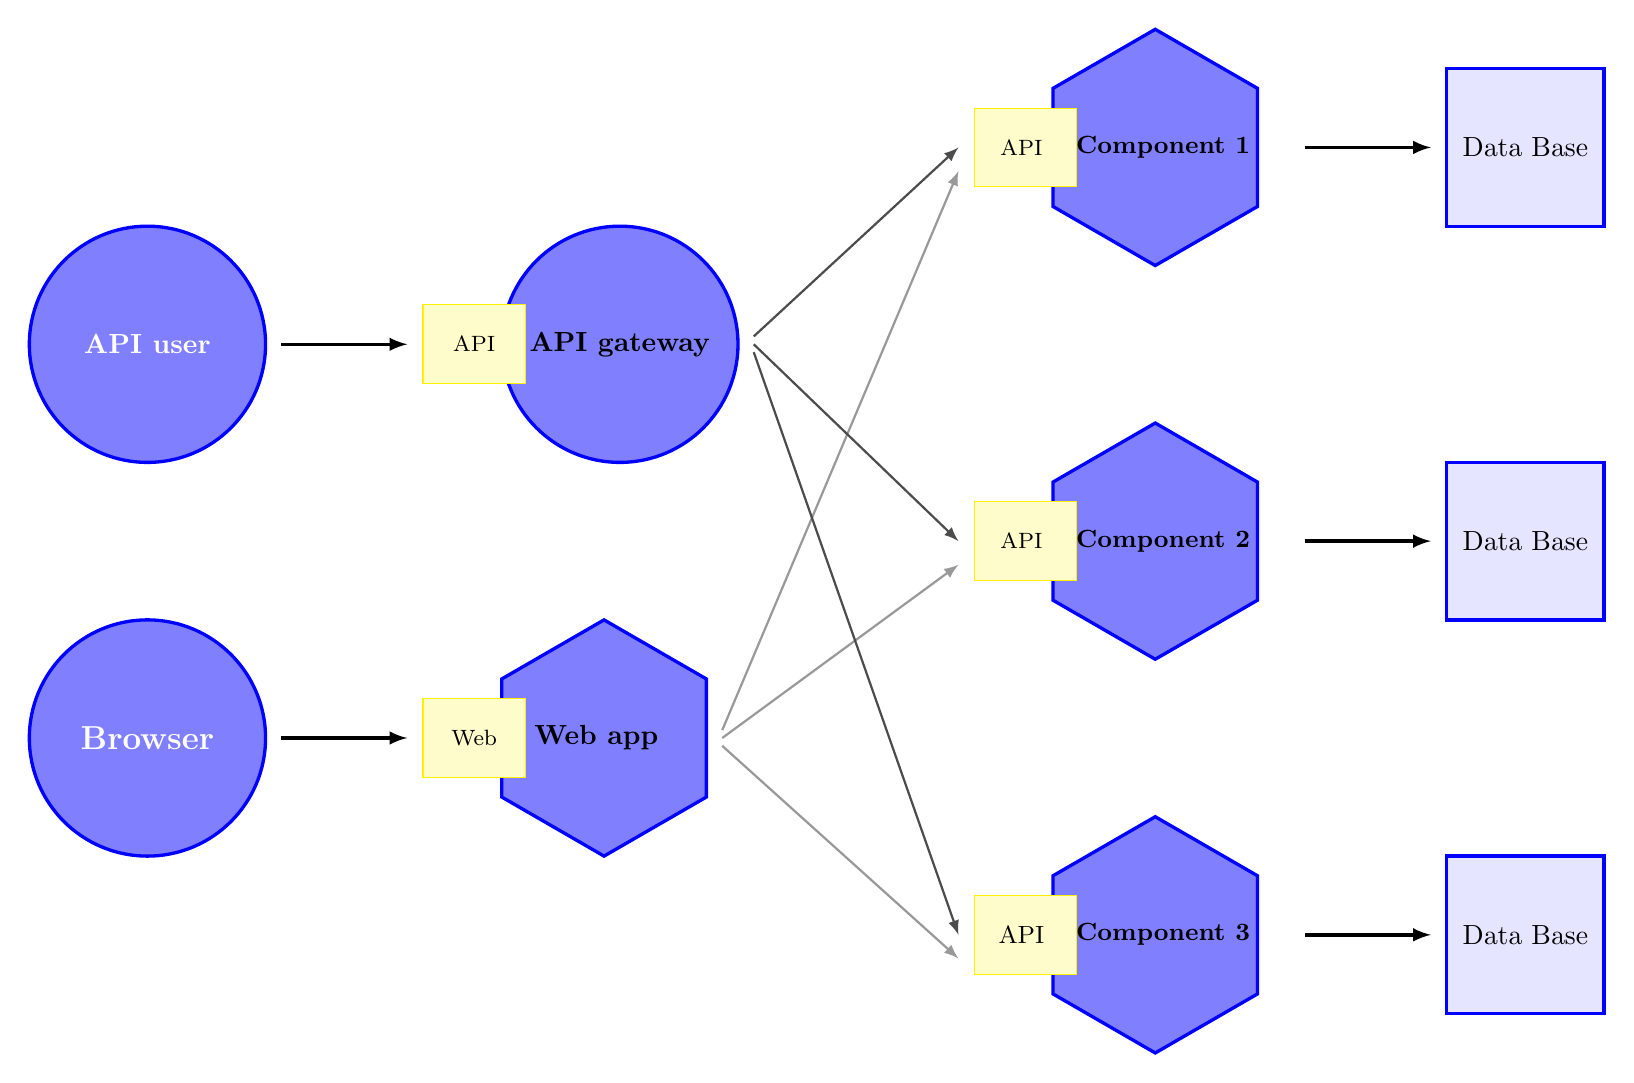
\begin{tikzpicture}

\draw [blue,fill=blue!50, very thick] (1.5,4) circle (1.5);
\draw (1.5,4) node[white] {\large{\textbf{Browser}}};
\draw [very thick, >=latex, ->] (3.2,4) -- (4.8,4);

\draw [blue,fill=blue!50, very thick] (1.5,9) circle (1.5);
\draw (1.5,9) node[white] {\textbf{API user}};
\draw [very thick, >=latex, ->] (3.2,9) -- (4.8,9);

\draw [blue,fill=blue!50, very thick] (6,4.75) -- (6,3.25)
-- ++(-30:1.5) -- ++(30:1.5) -- ++(90:1.5) -- ++(150:1.5) -- cycle;
\draw (7.2,4) node {\textbf{Web app}};
\draw [black!40, thick, >=latex, ->] (8.8,4.1) -- (11.8,11.2);
\draw [black!40, thick, >=latex, ->] (8.8,4) -- (11.8,6.2);
\draw [black!40, thick, >=latex, ->] (8.8,3.9) -- (11.8,1.2);
\draw [yellow,fill=yellow!20] (5,4.5) rectangle (6.3,3.5);
\draw (5.65,4) node {\footnotesize{Web}};

\draw [blue,fill=blue!50, very thick] (7.5,9) circle (1.5);
\draw (7.5,9) node {\textbf{API gateway}};
\draw [black!70, thick, >=latex, ->] (9.2,9.1) -- (11.8,11.5);
\draw [black!70, thick, >=latex, ->] (9.2,9) -- (11.8,6.5);
\draw [black!70, thick, >=latex, ->] (9.2,8.9) -- (11.8,1.5);
\draw [yellow,fill=yellow!20] (5,9.5) rectangle (6.3,8.5);
\draw (5.65,9) node {\footnotesize{API}};

\draw [blue,fill=blue!50, very thick] (13,12.25) -- (13,10.75)
-- ++(-30:1.5) -- ++(30:1.5) -- ++(90:1.5) -- ++(150:1.5) -- cycle;
\draw (14.4,11.5) node {\small{\textbf{Component 1}}};
\draw [very thick, >=latex, ->] (16.2,11.5) -- (17.8,11.5);
\draw [yellow,fill=yellow!20] (12,12) rectangle (13.3,11);
\draw (12.6,11.5) node {\footnotesize{API}};
\draw [blue,fill=blue!10, very thick] (18,12.5) rectangle (20,10.5);
\draw (19,11.5) node {Data Base};

\draw [blue,fill=blue!50, very thick] (13,7.25) -- (13,5.75)
-- ++(-30:1.5) -- ++(30:1.5) -- ++(90:1.5) -- ++(150:1.5) -- cycle;
\draw (14.4,6.5) node {\small{\textbf{Component 2}}};
\draw [very thick, >=latex, ->] (16.2,6.5) -- (17.8,6.5);
\draw [yellow,fill=yellow!20] (12,7) rectangle (13.3,6);
\draw (12.6,6.5) node {\footnotesize{API}};
\draw [blue,fill=blue!10, very thick] (18,7.5) rectangle (20,5.5);
\draw (19,6.5) node {Data Base};

\draw [blue,fill=blue!50, very thick] (13,2.25) -- (13,0.75)
-- ++(-30:1.5) -- ++(30:1.5) -- ++(90:1.5) -- ++(150:1.5) -- cycle;
\draw (14.4,1.5) node {\small{\textbf{Component 3}}};
\draw [very thick, >=latex, ->] (16.2,1.5) -- (17.8,1.5);
\draw [yellow,fill=yellow!20] (12,2) rectangle (13.3,1);
\draw (12.6,1.5) node {\small{API}};
\draw [blue,fill=blue!10, very thick] (18,2.5) rectangle (20,0.5);
\draw (19,1.5) node {Data Base};

\end{tikzpicture}

\end{document}
